Esta sección del apéndice fue tomado del trabajo de grado de Michael Stiven Honores Quishpillo y Juan David Naranjo Sánchez titulado "Propuesta de Transformación Digital para la Gestión de la Información en el Proceso de Producción Establecido en la Organización Prefabricados JAMAR Validada a través de la Construcción de un Prototipo Funcional". 

\subsection{elementos de negocio}

\begin{longtable}{|c|p{8cm}|}
\caption{Elementos de negocio en ArchiMate} \label{tab:elementos-negocio-archimate} \\
\hline
\textbf{Icono} & \textbf{Descripción} \\
\hline
\endfirsthead

\caption[]{Elementos de negocio en ArchiMate (continuación)} \\
\hline
\textbf{Icono} & \textbf{Descripción} \\
\hline
\endhead

\hline
\endfoot

\endlastfoot

\includegraphics{apendices/ARCHI/business/actor.png} & 
\textbf{Business Actor:} Una entidad que puede realizar un comportamiento dentro de la empresa, como una persona o una organización. \\
\hline
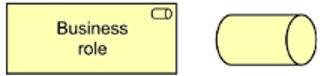
\includegraphics{apendices/ARCHI/business/rol.png} & 
\textbf{Business Role:} Define el conjunto de responsabilidades y comportamientos que un actor de negocio puede desempeñar. \\
\hline
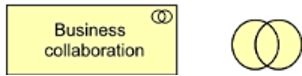
\includegraphics{apendices/ARCHI/business/colaboration.png} & 
\textbf{Business Collaboration:} Una agregación de dos o más roles de negocio que trabajan juntos para alcanzar un objetivo común. \\
\hline
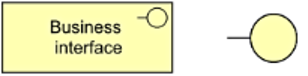
\includegraphics{apendices/ARCHI/business/interface.png} & 
\textbf{Business Interface:} Un punto de acceso donde un servicio de negocio es provisto a los actores de negocio. \\
\hline

\includegraphics{apendices/ARCHI/business/process.png} & 
\textbf{Business Process:} Un conjunto de actividades que logran un resultado específico para un cliente interno o externo. \\
\hline
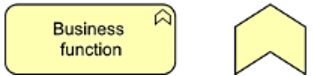
\includegraphics{apendices/ARCHI/business/function.png} & 
\textbf{Business Function:} Una agrupación de comportamientos con una base similar de recursos. \\
\hline

\includegraphics{apendices/ARCHI/business/interaction.png} & 
\textbf{Business Interaction:} Un comportamiento que describe la interacción entre dos o más roles de negocio. \\
\hline

\includegraphics{apendices/ARCHI/business/service.png} & 
\textbf{Business Service:} Un servicio que satisface una necesidad de un cliente, interno o externo, de la empresa. \\
\hline

\includegraphics{apendices/ARCHI/business/event.png} & 
\textbf{Business Event:} Algo que sucede y que afecta la continuidad de un proceso de negocio. \\
\hline
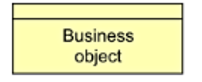
\includegraphics{apendices/ARCHI/business/object.png} & 
\textbf{Business Object:} Un concepto usado dentro de un dominio de negocio particular. \\
\hline
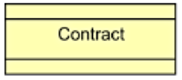
\includegraphics{apendices/ARCHI/business/contract.png} & 
\textbf{Contract:} Un acuerdo formal o informal que especifica los derechos y obligaciones asociados con un producto. \\
\hline
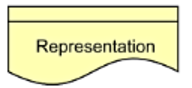
\includegraphics{apendices/ARCHI/business/representation.png} & 
\textbf{Representation:} Una forma perceptible de la información llevada por un objeto de negocio. \\
\hline
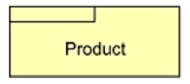
\includegraphics{apendices/ARCHI/business/product.png} & 
\textbf{Product:} Una colección coherente de servicios y/o objetos pasivos, acompañada de un contrato/conjunto de acuerdos. \\
\hline
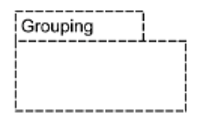
\includegraphics{apendices/ARCHI/business/grouping.png} &
\textbf{Grouping:} Un mecanismo para agrupar elementos relacionados en un modelo de arquitectura. \\
\end{longtable}

\subsection{elementos de aplicación}


